\section{Method}

SPRM converts outcome-only trajectory rewards into trainable step-level
supervision by separating two questions that are often conflated:
how much a step helps the current trajectory, and how valuable the underlying
reasoning pattern is across trajectories.
We instantiate the first question with a local credit signal derived from a
trajectory-level value scorer, and the second with a global semantic prior
estimated from the training corpus.
These two signals are then distilled into a dual-head process reward model.

\begin{figure*}[t]
\centering
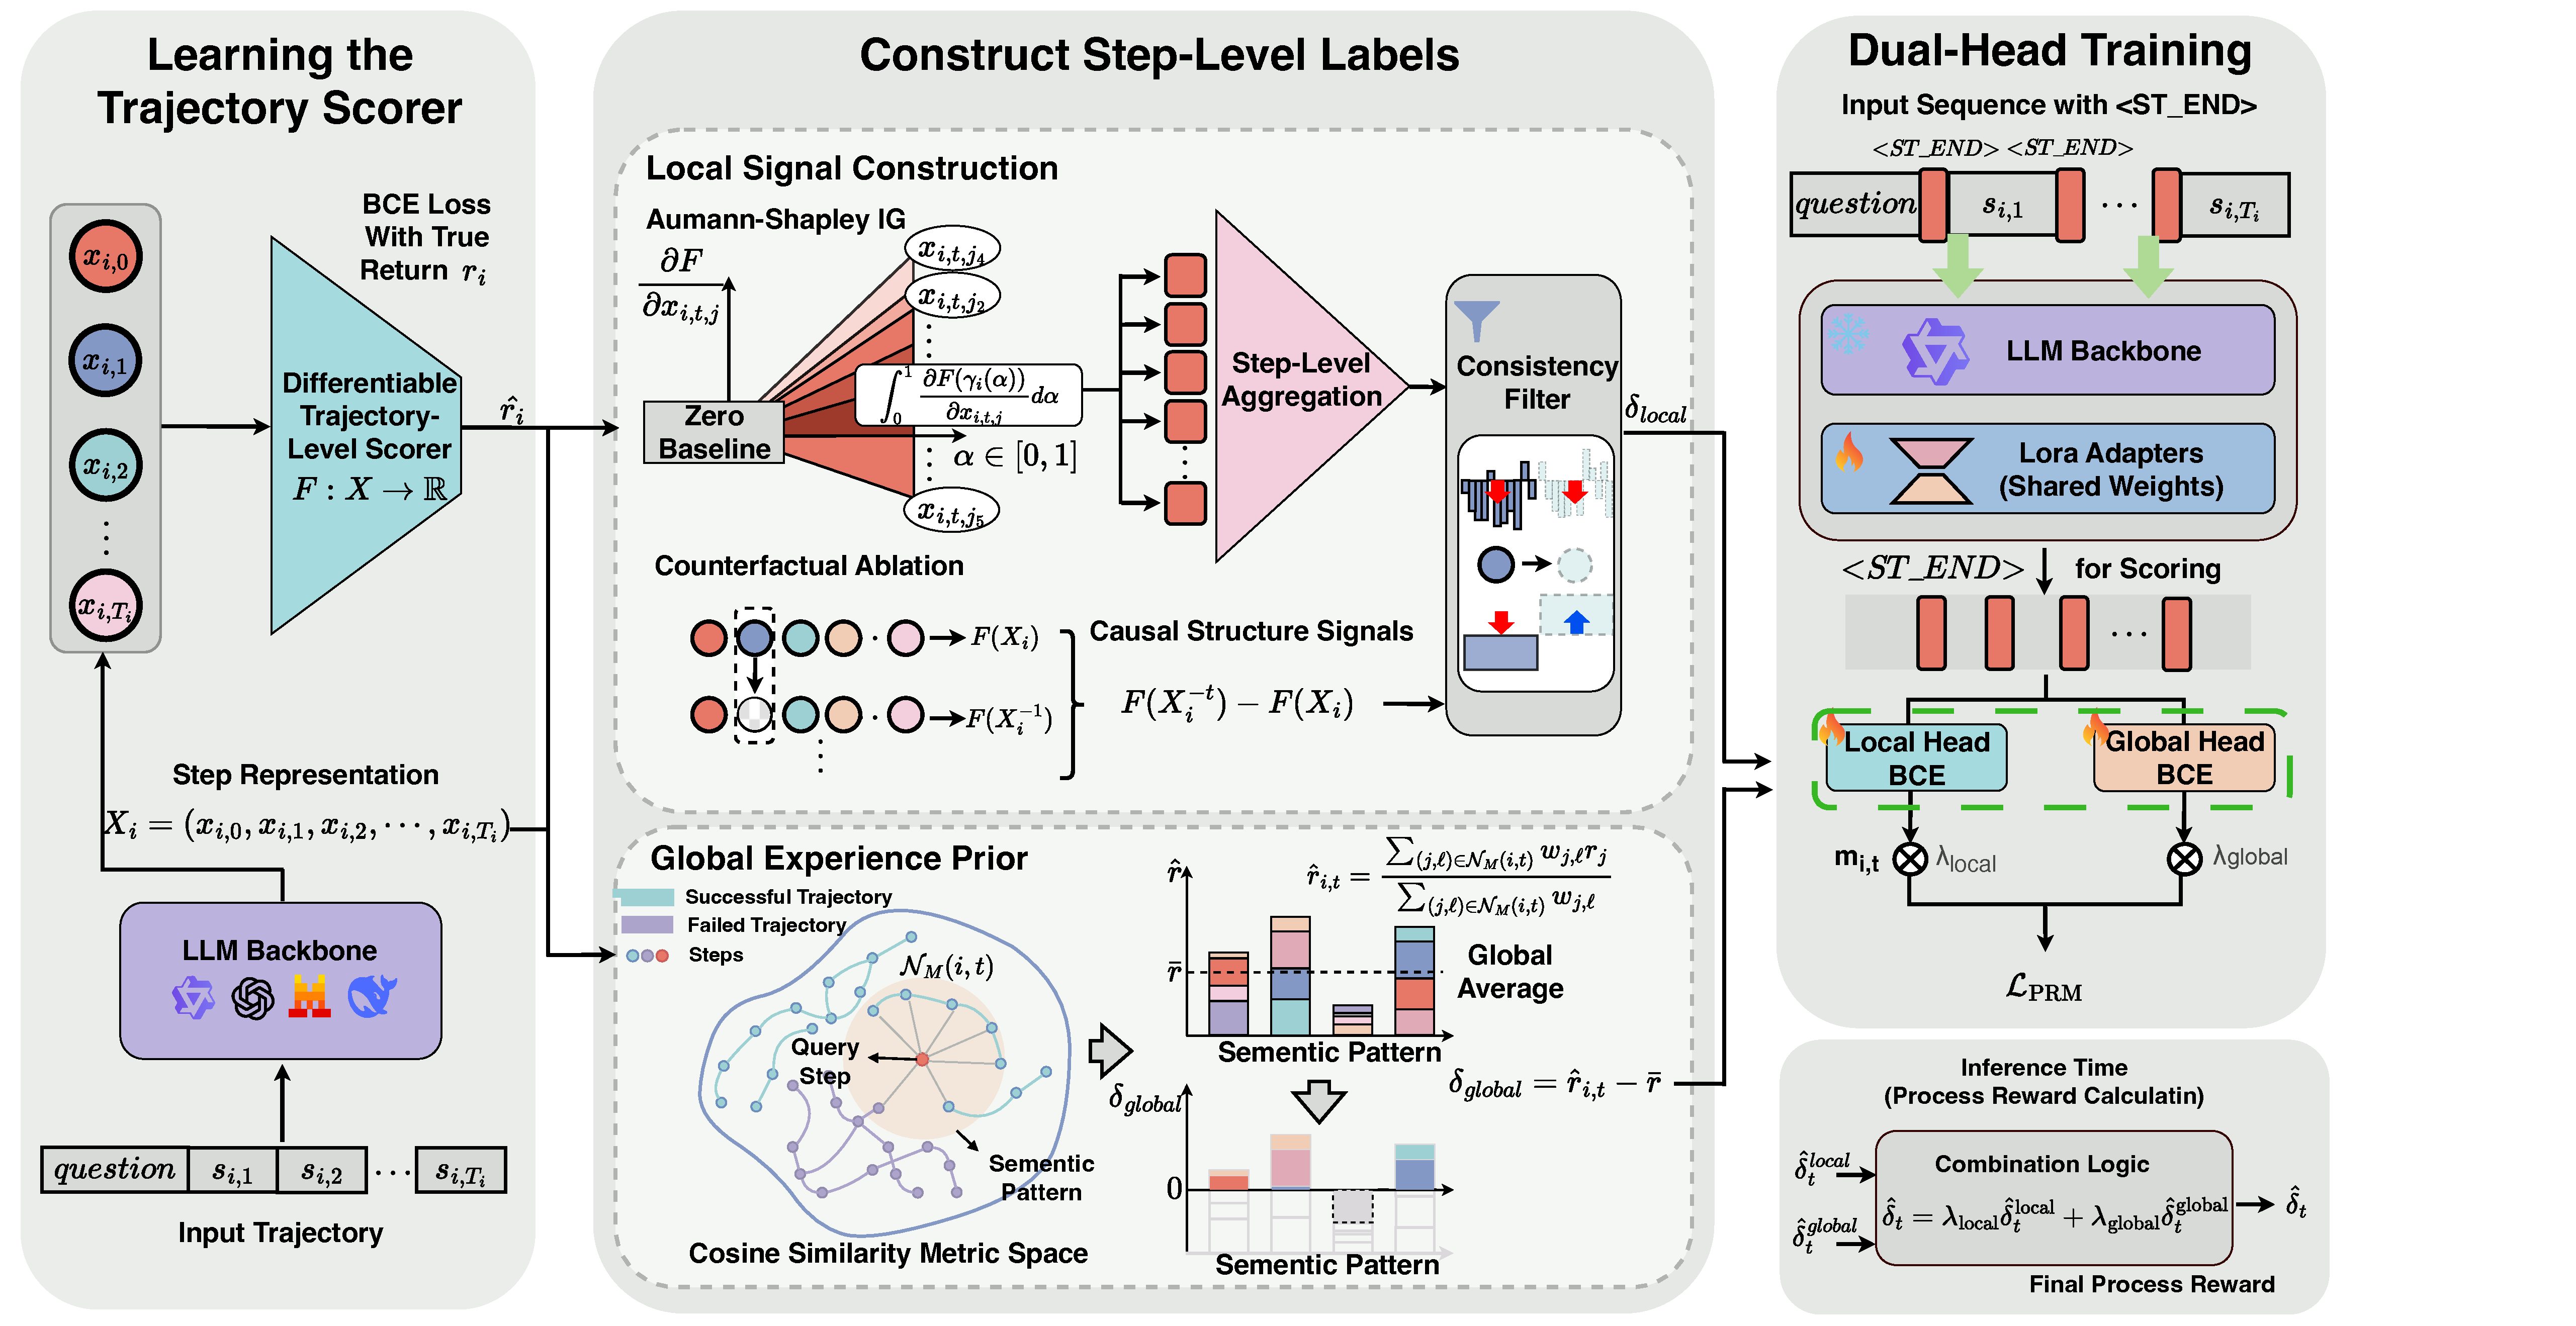
\includegraphics[width=\textwidth]{figures/overview-4-12.drawio.pdf}
\caption{Overview of SPRM.
Starting from outcome-only reasoning trajectories, we first encode the
question and each reasoning step into boundary representations.
We then construct two complementary supervision signals: a local signal from a
trajectory-level value proxy via Aumann--Shapley attribution and
counterfactual consistency checking, and a global signal from semantic
neighbor statistics across trajectories.
Both signals are finally distilled into a dual-head process reward model,
whose predictions are combined at inference time to produce the final
step-level reward.}
\label{fig:sprm_overview}
\end{figure*}

\subsection{Problem Setup and Overview}

Let
\(
\mathcal{D}=\{(\tau_i,r_i)\}_{i=1}^{N}
\)
be a dataset of reasoning trajectories, where
\(
\tau_i=(q_i,s_{i,1},\ldots,s_{i,T_i})
\)
contains a question \(q_i\), a sequence of reasoning steps
\(s_{i,1},\ldots,s_{i,T_i}\), and a final reward \(r_i\in[0,1]\).
Our goal is to transform this sparse trajectory-level signal into step-level
supervision for process reward modeling, without human step annotation,
per-step rollouts, or external judges at labeling time.

To represent each segment in a unified way, we insert a special boundary token
\(\langle\texttt{ST\_END}\rangle\) after the question and after every
reasoning step, and use the final-layer hidden state at each boundary position
as the representation of the immediately preceding segment.
Let \(x_{i,t}\in\mathbb{R}^{d}\) denote the boundary representation of segment
\(t\) in trajectory \(i\), where \(x_{i,0}\) is the question-boundary state.
We write the full boundary sequence as
\(
X_i=[x_{i,0},x_{i,1},\ldots,x_{i,T_i}]
\).
The encoder that maps \(\tau_i\) to \(X_i\) is the same backbone used to read
the full sequence with inserted boundary tokens; implementation details are
deferred to the appendix.

Figure~\ref{fig:sprm_overview} summarizes the full pipeline.
We first train a trajectory-level scorer to predict final rewards from complete
boundary sequences.
This scorer provides a differentiable value surface for local credit
assignment.
We then construct a local supervision signal from ordered attribution and
counterfactual consistency, and a global supervision signal from semantic
neighbor statistics across trajectories.
Finally, both signals are distilled into a shared PRM backbone with separate
local and global heads.

\subsection{Design Principle: Contextual Credit and Intrinsic Value}

The design of SPRM starts from a basic decomposition of step quality.
A reasoning step has a \emph{contextual contribution}, namely whether it
promotes or suppresses success in the specific trajectory where it appears, and
an \emph{intrinsic value}, namely whether the underlying reasoning pattern
tends to be useful across trajectories.
These two notions should not be conflated:
a helpful step can appear inside a failed trajectory, while a flawed step can
be locally masked inside a successful one.
SPRM therefore constructs two supervision signals that target these two
quantities separately.

For local credit, temporal order is part of the target quantity.
Given a trajectory \(\tau=(s_1,\dots,s_T)\), later steps depend on earlier
ones, so the observed order is the only causally valid order.
Under this constraint, the Shapley intuition reduces to an ordered marginal
view,
\begin{equation}
\label{eq:ordered_shapley_method}
\phi_t^{\mathrm{ord}}
:=
v_t-v_{t-1},
\qquad
v_t:=v(\{1,2,\dots,t\}),
\;
v_0:=v(\emptyset).
\end{equation}
Equation~\eqref{eq:ordered_shapley_method} motivates our local signal:
it should estimate how the current step changes trajectory value under the
observed reasoning order.
In practice, a single discrete difference is too brittle to serve as the final
supervision target by itself, so we use Aumann--Shapley attribution as a
continuous relaxation of ordered credit assignment and pair it with a discrete
counterfactual check.

The global signal answers a different question.
Its object is not a position in one trajectory, but a semantic reasoning
pattern that may recur across many trajectories.
For such patterns, the relevant quantity is closer to a distribution-level main
effect than to an ordered within-trajectory marginal.
If \(z\) denotes one semantic pattern, the ideal quantity is the main effect
\begin{equation}
\label{eq:global_main_effect_method}
\phi^{\mathrm{main}}(z)
:=
v(\{z\})-v(\emptyset),
\end{equation}
which measures how useful the pattern is relative to a global baseline.
Our global prior will be a practical approximation to this quantity using KNN
statistics in representation space.

\subsection{Local Supervision from a Trajectory-Level Value Proxy}

\subsubsection{Learning a differentiable trajectory scorer}

The local signal must evaluate a step in the context of the entire reasoning
chain.
Because the observed reward is defined only for complete trajectories, we first
learn a differentiable scorer
\(F_{\theta_{\mathrm{scorer}}}\) over full boundary sequences.
Given \(X_i\), the scorer predicts a final value
\(F_{\theta_{\mathrm{scorer}}}(X_i)\in[0,1]\).
We train it from trajectory-level supervision by minimizing
\begin{equation}
\label{eq:stage1_objective}
\mathcal{L}_{\mathrm{scorer}}(\theta_{\mathrm{scorer}})
=
\mathbb{E}_{(\tau,r)\sim\mathcal{D}}
\left[
\ell\!\left(F_{\theta_{\mathrm{scorer}}}(X),r\right)
\right],
\end{equation}
where \(\ell(\cdot,\cdot)\) is binary cross-entropy.
After training,
\(F_{\theta_{\mathrm{scorer}}^\star}\) serves as the value proxy used for local
credit construction.

\subsubsection{Continuous local credit via Aumann--Shapley attribution}

To quantify the contextual contribution of step \(s_{i,t}\), we measure how
the predicted final value changes when the full trajectory moves from a neutral
reference to the observed boundary sequence.
Let \(b\in\mathbb{R}^{d}\) be a baseline representation and
\(
B_i=[b,b,\ldots,b]
\)
the corresponding baseline sequence with the same length as \(X_i\).
Using the same baseline for continuous attribution and discrete ablation keeps
both local views in the same reference system.

We consider the interpolation path
\(
\gamma_i(\alpha)=B_i+\alpha(X_i-B_i)
\)
for \(\alpha\in[0,1]\).
The local continuous credit assigned to step \(s_{i,t}\) is
\begin{equation}
\label{eq:delta_local}
\delta_{\mathrm{local}}(s_{i,t})
=
\left(x_{i,t}-b\right)^\top
\int_0^1
\nabla_{x_{i,t}}
F_{\theta_{\mathrm{scorer}}^\star}(\gamma_i(\alpha))
\,d\alpha.
\end{equation}
This is the Aumann--Shapley attribution of the current step under the full
trajectory context.
It serves as our primary local supervision signal because it provides a smooth,
differentiable estimate of ordered marginal credit rather than relying on a
single hard ablation.

\subsection{Pairwise Counterfactual Consistency for Dependency-Aware Credit}

Continuous attribution alone does not directly encode what happens when steps
are explicitly removed from the trajectory.
We therefore introduce a discrete counterfactual view and use it as an
auxiliary consistency signal.
Importantly, this is a model-based counterfactual construction defined by the
trained scorer and the baseline replacement operation; it is not intended to
recover a full real-world causal graph.

Let \(X_i^{(-t)}\) denote the trajectory obtained by replacing only
\(x_{i,t}\) with the baseline \(b\), and let \(X_i^{(-t,-u)}\) denote the
trajectory where both \(x_{i,t}\) and \(x_{i,u}\) are replaced.
We first define the direct effect of removing step \(t\) as
\begin{equation}
\label{eq:r_direct}
R_{i,t}^{\mathrm{dir}}
=
F_{\theta_{\mathrm{scorer}}^\star}(X_i)
-F_{\theta_{\mathrm{scorer}}^\star}(X_i^{(-t)}).
\end{equation}
A positive value means that deleting the current step lowers the predicted
trajectory value, so the step is supportive under the scorer.

To make this counterfactual view sensitive to local step dependencies, we also
model pairwise interactions with nearby preceding steps.
For \(u<t\), define
\begin{equation}
\label{eq:pairwise_interaction}
I_{i,t,u}
:=
F_{\theta_{\mathrm{scorer}}^\star}(X_i)
-F_{\theta_{\mathrm{scorer}}^\star}(X_i^{(-t)})
-F_{\theta_{\mathrm{scorer}}^\star}(X_i^{(-u)})
+F_{\theta_{\mathrm{scorer}}^\star}(X_i^{(-t,-u)}).
\end{equation}
Positive \(I_{i,t,u}\) indicates that steps \(u\) and \(t\) act
synergistically under the scorer, whereas negative values indicate redundancy
or substitution.

We restrict these interactions to a local ordered window
\begin{equation}
\label{eq:interaction_window}
\mathcal{W}(t)
:=
\{u \mid 1 \le u < t,\; t-u \le w\},
\end{equation}
where \(w\) is a small window size.
Within this window, we define non-parametric interaction weights
\begin{equation}
\label{eq:pairwise_gate}
\bar g_{i,t,u}
:=
\frac{
\mathbf{1}(u\in\mathcal{W}(t))\cdot \max(I_{i,t,u},0)
}{
\sum_{v\in\mathcal{W}(t)} \max(I_{i,t,v},0)+\epsilon
}.
\end{equation}
We keep only positive interactions so that the correction term captures
supportive step dependencies without overwhelming the direct effect.

The final dependency-aware local counterfactual credit is
\begin{equation}
\label{eq:r_causal}
R_{i,t}^{\mathrm{causal}}
:=
R_{i,t}^{\mathrm{dir}}
+\beta \sum_{u\in\mathcal{W}(t)} \bar g_{i,t,u}\, I_{i,t,u},
\end{equation}
where \(\beta\) controls the strength of the interaction correction.
This quantity is not used as a direct training label.
Instead, it provides a discrete consistency check for the sign of the
continuous local attribution in \eqref{eq:delta_local}.

\subsection{Global Supervision as a Semantic Main-Effect Prior}

Local attribution estimates how a step functions inside one trajectory, but a
step also instantiates a reasoning pattern whose value may persist across many
contexts.
We capture this second aspect with a global semantic prior estimated directly
from the dataset.
From the perspective of
\eqref{eq:global_main_effect_method}, the goal is to approximate the main
effect of the semantic pattern associated with the current step.

We do not define patterns manually.
Instead, each step induces a soft semantic neighborhood in representation
space.
For step \(s_{i,t}\), let \(\mathcal{N}_M(i,t)\) denote its top-\(M\)
nearest steps from other trajectories, and let \(w_{j,\ell}\ge 0\) be the
similarity-based weight assigned to neighbor \((j,\ell)\).
The neighborhood success estimate is
\[
\hat r(s_{i,t})
=
\frac{
\sum_{(j,\ell)\in\mathcal{N}_M(i,t)} w_{j,\ell}r_j
}{
\sum_{(j,\ell)\in\mathcal{N}_M(i,t)} w_{j,\ell}
}.
\]
Comparing this quantity with the dataset-wide average reward
\(
\bar r=\frac{1}{N}\sum_{i=1}^{N}r_i
\),
we define the global prior
\begin{equation}
\label{eq:delta_global}
\delta_{\mathrm{global}}(s_{i,t})
=
\hat r(s_{i,t})-\bar r.
\end{equation}
This quantity is a practical approximation to the main effect of the semantic
pattern associated with \(s_{i,t}\):
\(\hat r(s_{i,t})\) estimates how often similar patterns appear in successful
trajectories, while \(\bar r\) serves as the null baseline.
It therefore complements the local signal with a more stable
distribution-level prior.

\subsection{Distilling Local and Global Signals into the Process Reward Model}

We use the two constructed signals to supervise a final process reward model at
the same boundary positions.
The model reads the sequence with inserted
\(\langle\texttt{ST\_END}\rangle\) tokens and outputs one reward prediction per
boundary position.
We use a shared backbone with two task-specific heads, jointly parameterized by
\(\theta_{\mathrm{LLM}}\).
At step \(s_{i,t}\), the model predicts
\(\hat\delta_{i,t}^{\mathrm{local}}\) and
\(\hat\delta_{i,t}^{\mathrm{global}}\), trained against binarized targets
\(
\bar{\delta}_{i,t}^{\mathrm{local}}
=
\mathbf{1}(\delta_{\mathrm{local}}(s_{i,t})>0)
\)
and
\(
\bar{\delta}_{i,t}^{\mathrm{global}}
=
\mathbf{1}(\delta_{\mathrm{global}}(s_{i,t})>0)
\).

For the local head, we retain a step only when the continuous attribution and
the discrete counterfactual view agree on the direction of its effect.
We therefore define the consistency mask
\begin{equation}
\label{eq:local_mask}
m_{i,t}
:=
\mathbf{1}\!\left(
\delta_{\mathrm{local}}(s_{i,t})\cdot R_{i,t}^{\mathrm{causal}}>0
\right).
\end{equation}
The local loss is applied only when \(m_{i,t}=1\), which filters out noisy
steps where the two local views disagree.

The final training objective is
\begin{equation}
\label{eq:stage3_objective}
\begin{split}
\mathcal{L}_{\mathrm{PRM}}(\theta_{\mathrm{LLM}})
=
\mathbb{E}_{(\tau,r)\sim\mathcal{D}}
\Big[
&\lambda_{\mathrm{local}}
\sum_t
m_t\,
\mathrm{BCE}\!\left(
\hat{\delta}_t^{\mathrm{local}},
\bar{\delta}_t^{\mathrm{local}}
\right) \\
&+
\lambda_{\mathrm{global}}
\sum_t
\mathrm{BCE}\!\left(
\hat{\delta}_t^{\mathrm{global}},
\bar{\delta}_t^{\mathrm{global}}
\right)
\Big],
\end{split}
\end{equation}
where the local head captures trajectory-specific credit while the global head
injects a more stable semantic prior.

At inference time, we combine the two heads as
\(
\hat\delta_{i,t}
=
\lambda_{\mathrm{local}}\hat\delta_{i,t}^{\mathrm{local}}
+
\lambda_{\mathrm{global}}\hat\delta_{i,t}^{\mathrm{global}}.
\)
The resulting score balances contextual causal evidence with
cross-trajectory regularity and is used as the final step-level process reward.
